\subsection{使用 Q学习 解决悬崖寻路问题} 

强化学习在运动规划方面也有很大的应用前景,目前有很多对应的仿真环境,小到迷宫游戏,大到贴近真实的自动驾驶环境CARLA。本节使用OpenAI Gym开发的\kw{CliffWalking-v0}环境,带读者入门Q学习算法的代码实战。

\subsubsection{CliffWalking-v0 环境简介} 

我们首先简单介绍 CliffWalking-v0 环境,该环境中文名为悬崖寻路(cliff walking),是一个迷宫类问题。如\figref{fig:cliffwalking_ch3} 所示,在一个$4 \times 12$的网格中,智能体以网格的左下角位置为起点,以网格的右下角位置为终点,目标是移动智能体到达终点位置,智能体每次可以在上、下、左、右这4个方向中移动一步,每移动一步会得到 $-1$ 单位的奖励。

\begin{figure}[htb]
    \centering
    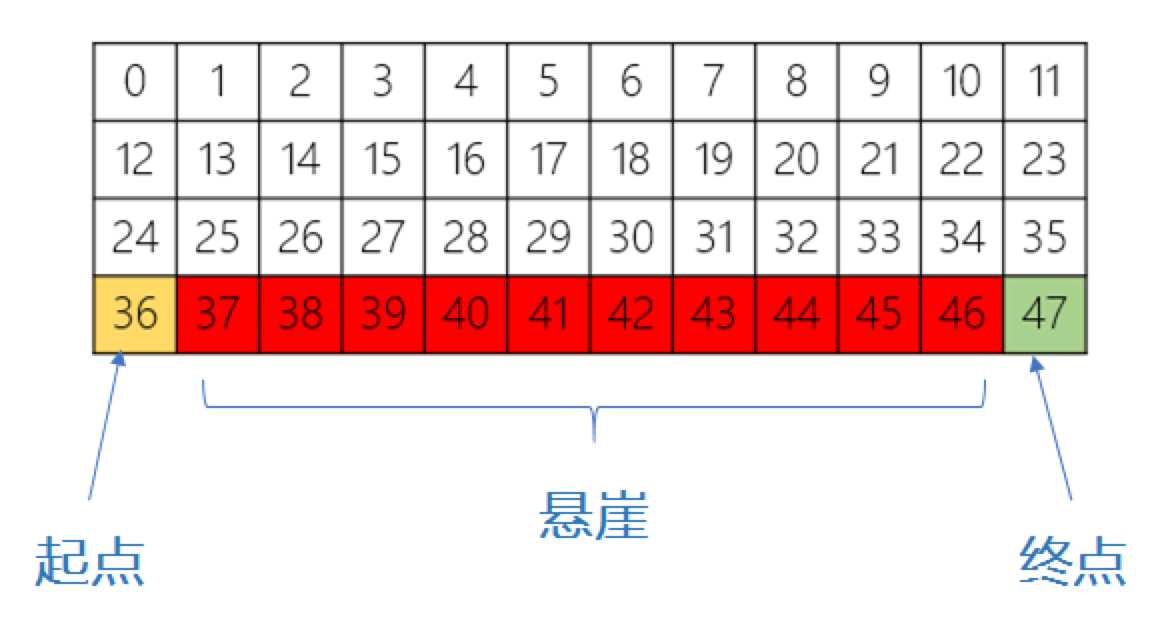
\includegraphics[width=0.5\linewidth]{res/ch3/assets/cliffwalking_1}
    \caption{CliffWalking-v0 环境}
    \label{fig:cliffwalking_ch3}
\end{figure}

起终点之间是一段悬崖,即编号为$37~46$的网格,智能体移动过程中会有如下的限制:

(1)智能体不能移出网格,如果智能体想执行某个动作移出网格,那么这一步智能体不会移动,但是这个操作依然会得到$-1$W单位的奖励;

(2)如果智能体“掉入悬崖” ,会立即回到起点位置,并得到$-100$单位的奖励;

(3)当智能体移动到终点时,该回合结束,该回合总奖励为各步奖励之和。

我们的目标是以最少的步数到达终点,容易看出最少需要$13$步智能体才能从起点到终点,因此最佳算法收敛的情况下,每回合的总奖励应该是$-13$,这样人工分析出期望的奖励也便于我们判断算法的收敛情况从而做出相应调整。现在我们可以在代码中定义环境,如下:

\begin{lstlisting}[style=Python]
    import gym # 导入gym模块
    from envs.gridworld_env import CliffWalkingWapper # 导入自定义装饰器
    env = gym.make('CliffWalking-v0')  # 定义环境
    env = CliffWalkingWapper(env) # 装饰环境
\end{lstlisting}

我们在程序中使用了一个装饰器重新定义环境,但不影响对环境的理解,感兴趣的同学具体看相关代码。由于 gym 环境封装得比较好,因此我们想要使用这个环境只需要使用 gym.make 命令输入函数名即可,然后我们就可以查看环境的状态和动作数:

\begin{lstlisting}[style=Python]
    n_states = env.observation_space.n # 状态数
    n_actions = env.action_space.n # 动作数
    print(f"状态数:{n_states},动作数:{n_actions}")
\end{lstlisting}

输出结果如下:
\begin{lstlisting}[language=sh,basicstyle=\zihao{-5}\ttfamily]
    状态数:48,动作数:4
\end{lstlisting}

我们的状态数是$48$,这里我们设置的是智能体当前所在网格的编号,而动作数是$4$,这表示有$0$、$1$、$2$、$3$这四个数对应上、右、下、左4个动作。另外我们也可以初始化环境并输出当前的状态:

\begin{lstlisting}[style=Python]
    state = env.reset()
    print(f"初始状态:{state}")
\end{lstlisting}

结果显示为:

\begin{lstlisting}[language=sh,basicstyle=\zihao{-5}\ttfamily] 
    初始状态:36
\end{lstlisting}

也就是当前智能体的状态即当前所在的网格编号$36$,正好对应我们前面讲到的起点。

\subsubsection{强化学习基本接口}

这里所说的接口是指一般强化学习的训练模式,也是大多数算法伪代码遵循的规则,步骤如下:

(1)初始化环境和智能体;

(2)对于每个回合,智能体选择动作;

(3)环境接收动作并反馈下一个状态和奖励;

(4)智能体进行策略更新(学习);

(5)多个回合之后算法收敛保存模型以及做后续的分析、画图等。

代码如下:

\begin{lstlisting}[style=Python]
    env = gym.make('CliffWalking-v0')  # 定义环境
    env = CliffWalkingWapper(env) # 装饰环境
    env.seed(1) # 设置随机种子
    n_states = env.observation_space.n # 状态数
    n_actions = env.action_space.n # 动作数
    agent = QLearning(n_states,n_actions,cfg) # cfg存储算法相关参数
    for i_ep in range(cfg.train_eps): # cfg.train_eps表示最大的训练回合数
        ep_reward = 0  # 记录每个回合的奖励
        state = env.reset()  # 重置环境
        while True: 
            action = agent.choose_action(state)  # 算法选择一个动作
            next_state, reward, done, _ = env.step(action)  # 环境根据动作反馈奖励和下一个状态
            agent.update(state, action, reward, next_state, done)  # 算法更新
            state = next_state  # 更新状态
            ep_reward += reward
            if done: # 终止状态
                break
\end{lstlisting}

通常我们会记录并分析奖励的变化,所以在接口基础上加一些变量以记录每回合的奖励。此外,由于强化学习训练过程中得到的奖励可能会产生振荡,因此我们也使用一个滑动平均的量来反映奖励变化的趋势,如下:

\begin{lstlisting}[style=Python]
    rewards = []  
    ma_rewards = [] # 滑动平均奖励
    for i_ep in range(cfg.train_eps):
        ep_reward = 0  # 记录每个回合的奖励
        state = env.reset()  # 重置环境, 重新开始(开始一个新的回合)
        while True:
            action = agent.choose_action(state)  # 根据算法选择一个动作
            next_state, reward, done, _ = env.step(action)  # 与环境进行一次动作交互
            agent.update(state, action, reward, next_state, done)  # Q学习算法更新
            state = next_state  # 存储上一个观察值
            ep_reward += reward
            if done:
                break
    rewards.append(ep_reward)
    if ma_rewards:
        ma_rewards.append(ma_rewards[-1]*0.9+ep_reward*0.1)
        else:
            ma_rewards.append(ep_reward)
\end{lstlisting}

\subsubsection{ Q 学习算法}

了解基本接口之后,现在我们看看 Q 学习算法具体是怎么实现的。前文讲到智能体在整个训练中只做两件事,一是选择动作,一是更新策略,所以我们可以定义一个 Qlearning 类,里面主要包含两个函数,即 choose\_action() 和 update() 。我们先看看 choose\_action() 函数是怎么定义的,如下:
\begin{lstlisting}[style=Python]
    def choose_action(self, state):
        self.sample_count += 1
        self.epsilon = self.epsilon_end + (self.epsilon_start - self.epsilon_end) * \
            math.exp(-1. * self.sample_count / self.epsilon_decay) # epsilon是会递减的,这里选择指数递减
        #  带有探索的贪心策略
        if np.random.uniform(0, 1) > self.epsilon:
            action = np.argmax(self.Q_table[str(state)]) # 选择Q(s,a)最大值对应的动作
        else:
            action = np.random.choice(self.action_dim) # 随机选择动作
        return action
\end{lstlisting}

一般我们使用$\varepsilon$-贪心策略选择动作。我们的输入就是当前的状态,随机选取一个值,当这个值大于我们设置的 epsilion 时,我们选取最大Q值对应的动作,否则随机选择动作,这样就能在训练中让智能体保持一定的探索率,这也是平衡探索与利用的技巧之一。

下面是我们要实现的策略更新函数:

\begin{lstlisting}[style=Python]
    def update(self, state, action, reward, next_state, done):
        Q_predict = self.Q_table[str(state)][action] 
        if done: # 终止状态
            Q_target = reward  
        else:
            Q_target = reward + self.gamma * np.max(self.Q_table[str(next_state)]) 
        self.Q_table[str(state)][action] += self.lr * (Q_target - Q_predict)
\end{lstlisting}

这里面实现的逻辑就是伪代码中的更新公式,如式\eqref{eq:ch3_ex_1}所示。

\begin{equation}
	Q(S, A) \leftarrow Q(S, A)+\alpha\left(R+\gamma \max _{a} Q\left(S^{\prime}, a\right)-Q(S, A)\right)
	\label{eq:ch3_ex_1}
\end{equation}

注意终止状态下,我们是获取不到下一个动作的,我们直接将 Q\_target 更新为对应的奖励即可。 

\subsubsection{结果分析}

到现在我们就基本完成了 Q 学习算法的代码实现,具体可以查看 GitHub 上的源码,代码运行结果如\figref{fig:train_rewards_curve_cn} 所示。

\begin{figure}[htb]
    \centering
    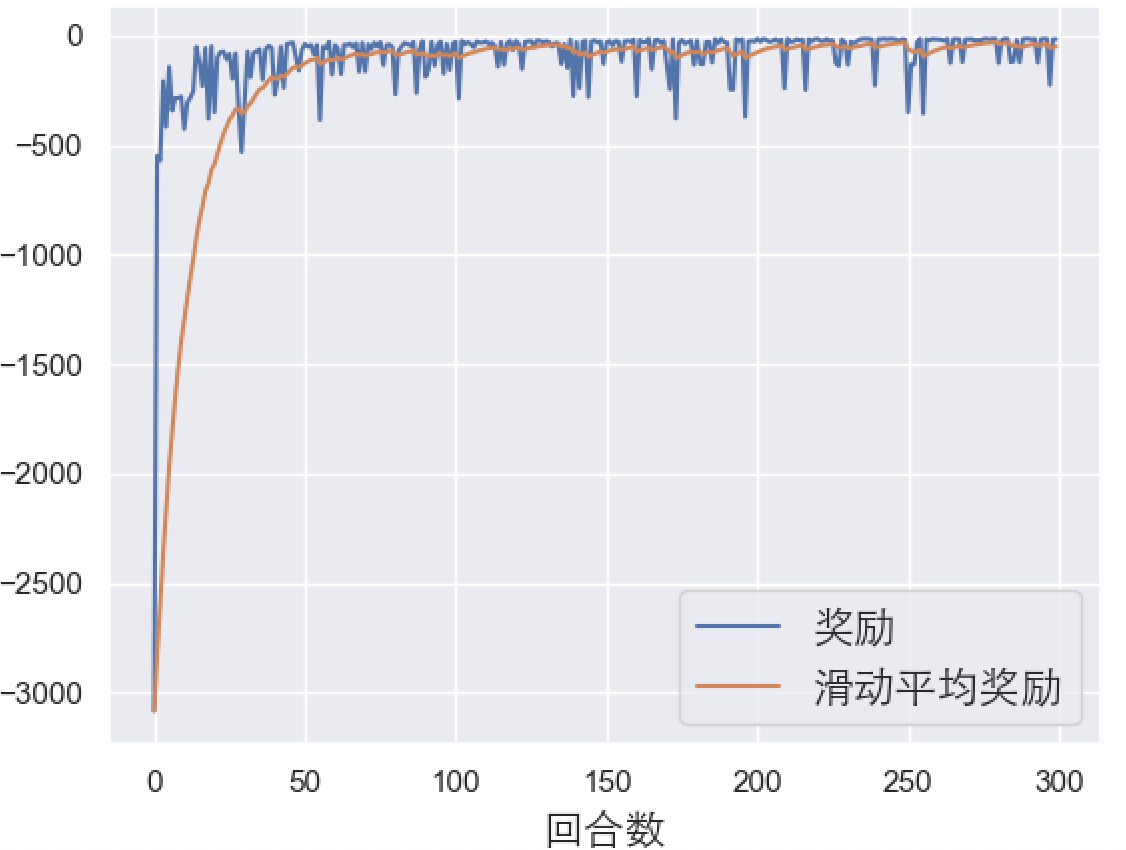
\includegraphics[width=0.5\linewidth]{res/ch3/assets/train_rewards_curve_cn}
    \caption{CliffWalking-v0 环境下 Q 学习算法的训练学习曲线}
    \label{fig:train_rewards_curve_cn}
\end{figure}

由于这个环境比较简单,因此可以看到算法很快达到收敛,然后我们再测试训练好的模型,一般测试模型只需要$20~50$左右的回合。

如\figref{fig:eval_rewards_curve_cn} 所示,这里我们测试的回合数为 30 ,可以看到每个回合智能体都得到了最优的奖励,说明我们算法的训练效果很不错!

\begin{figure}[htb]
    \centering
    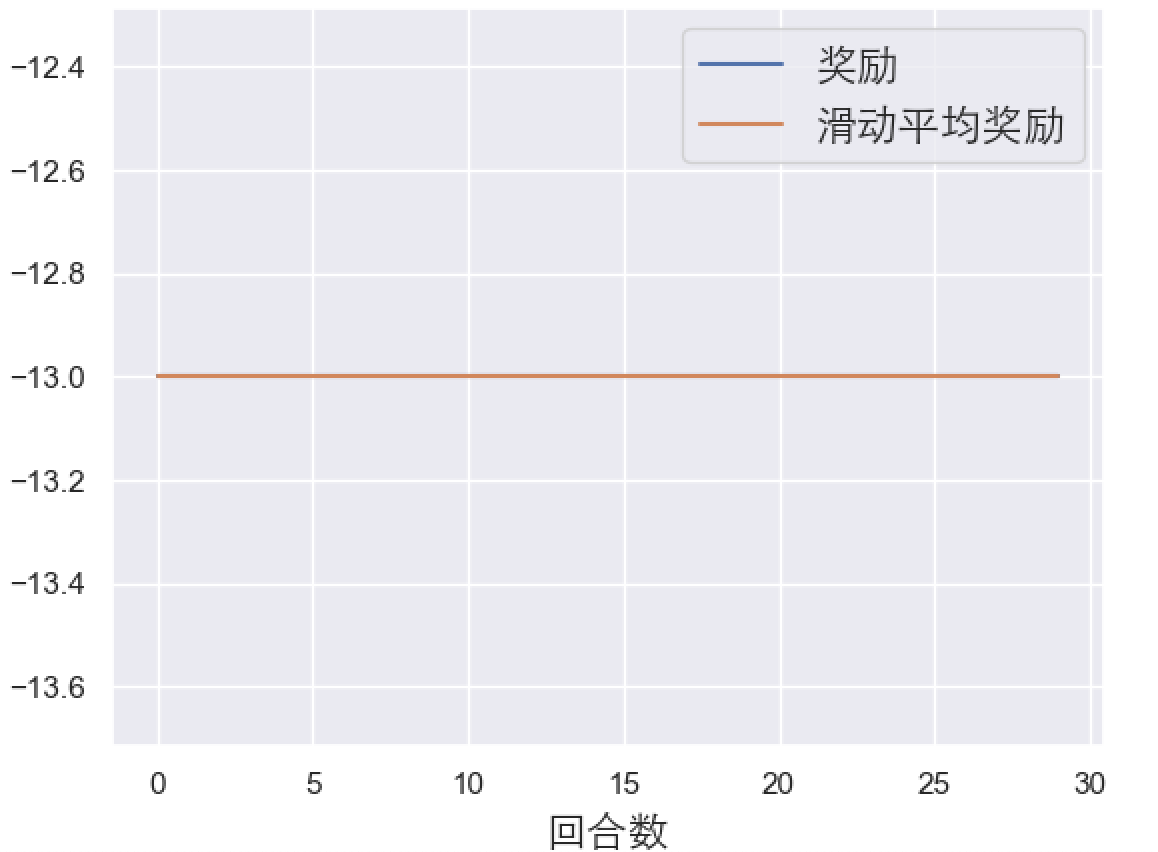
\includegraphics[width=0.5\linewidth]{res/ch3/assets/eval_rewards_curve_cn}
    \caption{CliffWalking-v0 环境下 Q 学习算法的测试学习曲线}
    \label{fig:eval_rewards_curve_cn}
\end{figure}
